\documentclass{beamer}
\beamertemplatenavigationsymbolsempty
\mode<presentation> {

%\usetheme{default}		%show
%\usetheme{AnnArbor}
%\usetheme{Antibes}
%\usetheme{Bergen}
%\usetheme{Berkeley}
%\usetheme{Berlin}
%\usetheme{Boadilla}
%\usetheme{CambridgeUS}	%show
%\usetheme{Copenhagen}
%\usetheme{Darmstadt}	%show
%\usetheme{Dresden}
%\usetheme{Frankfurt}
%\usetheme{Goettingen}
%\usetheme{Hannover}
%\usetheme{Ilmenau}
%\usetheme{JuanLesPins}
%\usetheme{Luebeck}
\usetheme{Madrid}
%\usetheme{Malmoe}
%\usetheme{Marburg}
%\usetheme{Montpellier}
%\usetheme{PaloAlto}
%\usetheme{Pittsburgh}
%\usetheme{Rochester}
%\usetheme{Singapore}	%show
%\usetheme{Szeged}
%\usetheme{Warsaw}

% As well as themes, the Beamer class has a number of color themes
% for any slide theme. Uncomment each of these in turn to see how it
% changes the colors of your current slide theme.

%\usecolortheme{albatross}
%\usecolortheme{beaver}
%\usecolortheme{beetle}
%\usecolortheme{crane}
%\usecolortheme{dolphin}
%\usecolortheme{dove}
%\usecolortheme{fly}
%\usecolortheme{lily}
%\usecolortheme{orchid}
%\usecolortheme{rose}
%\usecolortheme{seagull}
%\usecolortheme{seahorse}
%\usecolortheme{whale}
%\usecolortheme{wolverine}

%\setbeamertemplate{footline} % To remove the footer line in all slides uncomment this line
%\setbeamertemplate{footline}[page number] % To replace the footer line in all slides with a simple slide count uncomment this line

%\setbeamertemplate{navigation symbols}{} % To remove the navigation symbols from the bottom of all slides uncomment this line
}

\usepackage{graphicx} % Allows including images
\usepackage{booktabs} % Allows the use of \toprule, \midrule and \bottomrule in tables
\usepackage{smartdiagram}
\usepackage{tikz}
\usetikzlibrary{shapes.geometric, arrows}
\tikzstyle{startstop} = [rectangle, rounded corners, minimum width=3cm, minimum height=1cm,text centered, draw=black, fill=red!30]
\tikzstyle{io} = [trapezium, trapezium left angle=70, trapezium right angle=110, minimum width=3cm, minimum height=1cm, text centered, draw=black, fill=blue!30]
\tikzstyle{process} = [rectangle, minimum width=3cm, minimum height=1cm, text centered, draw=black, fill=orange!30]
\tikzstyle{decision} = [diamond, minimum width=3cm, minimum height=1cm, text centered, draw=black, fill=green!30]
\tikzstyle{arrow} = [thick,->,>=stealth]


\newcommand{\rank}[1]{\textnormal{rk}\left(#1\right)}

\title[]{Why you should not kick me out of my PhD (yet)} % The short title appears at the bottom of every slide, the full title is only on the title page

\author{Dominic Maderazo} % Your name
%\institute[UCLA] % Your institution as it will appear on the bottom of every slide, may be shorthand to save space
{
%Monash University\\ % Your institution for the title page
\medskip
%\textit{john@smith.com} % Your email address
}
\date{\today} % Date, can be changed to a custom date

\begin{document}
    \begin{frame}
        \titlepage 
    \end{frame}
    
    % \begin{frame}{Plan}
    %     Dunno how long this should be
        
    %     \begin{itemize}
    %         \item Sequence segmentation: an example
    %         \item Transcription Factor Binding Sites
    %         \item Enhancers
    %         \item Bayesian Segmentation and classification
    %         \item GGS (Perhaps a bonus slide)
    %         \item Binary classifiers and optimal combinations
    %         \item Incorporating new data
    %         \item Alignment Free methods?
    %     \end{itemize}
    % \end{frame}
    
    % \begin{frame}{Sequence Segmentation}
    %     Chop up some lines! 
    %     \begin{block}{Problem:}
    %         \begin{itemize}
    %             \item 2 coins, with $\theta_1$ and $\theta_2$ probability of showing heads 
    %             \item Dealer flips coin 1 $k_1$ times and then changes to coin 2 and flips $k_2$ times
    %             \item Given nothing but the sequence of residues, can we work out:
    %                 \begin{itemize}
    %                     \item $\theta_1, \theta_2$
    %                     \item $k_1,k_2$
    %                     \item $A_k$ position in the sequence when the dealer changed coins
                        
    %                 \end{itemize}
    %         \end{itemize}
    %     \end{block}
    % \end{frame}
    
    \begin{frame}{Central Dogma of Molecular Biology}
    \centering
    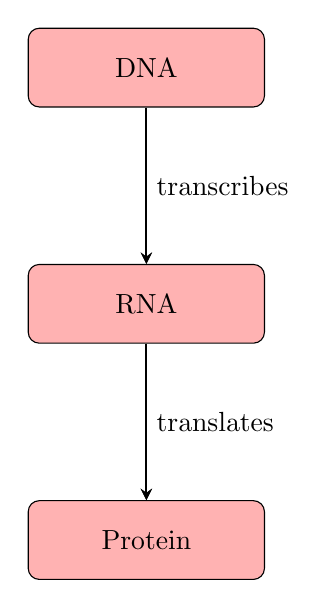
\begin{tikzpicture}[node distance=3cm]
        \node (DNA) [startstop]{DNA};
        \node (RNA) [startstop, below of = DNA]{RNA};
        \node (Protein) [startstop, below of = RNA]{Protein};
        
        \draw[arrow] (DNA) -- (RNA);
        \draw[arrow] (RNA) -- (Protein);
        
        \draw [arrow] (DNA) -- node[anchor=west] {transcribes} (RNA);
\draw [arrow] (RNA) -- node[anchor=west] {translates} (Protein);
    \end{tikzpicture}
        
    \end{frame}
    \begin{frame}{Transcription Factors}
        \begin{block}{Transcription Factors (TFs)}
            Proteins involved in the process of converting, or transcribing, DNA into RNA.
        \end{block}
        
        \begin{block}{TF Binding Site (TFBS)}
            Short stretch of DNA, 6-8 base pairs (bp) for TF binding.
        \end{block}
        \begin{block}{Enhancers}
            DNA regulatory sequences that can be bound to by TFs that help regulate the transcription process
        \end{block}
        
        \pause
         \begin{block}{Aim:}
         Identification of these enhancer regions.
         \end{block}
    \end{frame}
    
    \begin{frame}{A Picture}
        \begin{figure}
            \centering
            
\includegraphics[width = 0.9\textwidth]{tfBinding.pdf}
            \caption{Yeet}
            \label{fig:yeet}
        \end{figure}
    \end{frame}
    % \begin{frame}{Enhancers}
    %     What do enhancers do? They kinda are a special type of TFBS
    % \end{frame}
    
    \begin{frame}{Chromatin}
        DNA is stored by being wrapped around protein structures called histones, making up what is known as \textbf{chromatin}.
        \begin{figure}
            \centering
            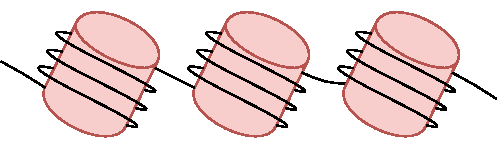
\includegraphics{Chromatin.pdf}
            \caption{Wrapping snakes around marshmallows makes for a delicious treat}
            \label{fig:chromatin}
        \end{figure}
    \end{frame}
    
    \begin{frame}{More pictures}
        \begin{figure}
            \centering
            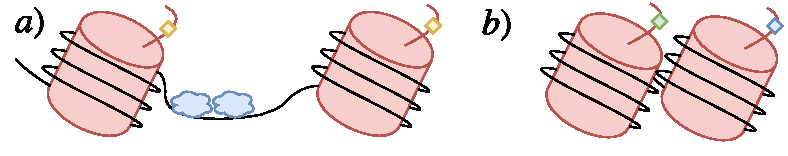
\includegraphics[width = \textwidth]{OpenCloseChromatinEpi.pdf}
            \caption{yote}
            \label{fig:yote}
        \end{figure}
    \end{frame}
    
    \begin{frame}{Sequence Segmentation}
        \begin{figure}
            \centering
            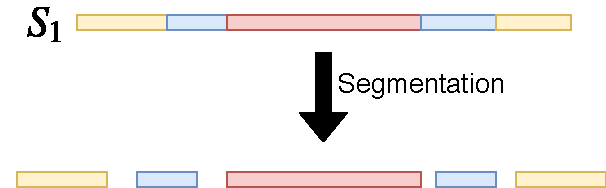
\includegraphics{Segmentation.pdf}
            \caption{Yate}
            \label{fig:Segmentation}
        \end{figure}
    \end{frame}
    \begin{frame}{Sequence Segmentation}
       % Given a sequence $S$ generated by 2 coins of different biases. 
       Consider a game where an opponent: 
        \begin{itemize}
            \item has 2 coins with probability of showing heads $\theta_1$ and $\theta_2$ ($\theta_1\neq\theta_2$).
            \item flips one coin $c$ times and then switches over to the second coin.
        
        \end{itemize}
        
        \pause 
        Given only the final sequence $S$ and the number of change points, infer:
        \begin{block}{}
            \begin{itemize}
               % \item 2 coins with probability of showing heads $\theta_1$ and $\theta_2$ ($\theta_1\neq\theta_2$)
                %\item Dealer flips coin 1 $k_1$ times and then changes to coin 2 and flips $k_2$ times
                %\item Given nothing but the sequence of residues and the number of coins:
                    %\begin{itemize}
                        \item The biases of the coins $\theta_1, \theta_2$
                        
                        \item The point at which the coins were exchanged $c$ (i.e. the change point)
                        
                    %\end{itemize}
            \end{itemize}
        \end{block}
    \end{frame}
    
    \begin{frame}{Bayesian Segmentation}
        Assuming the outcomes of the residues are independent, we have that:  
            \begin{block}{Likelihood}
            $P(S, C = c|\theta_1,\theta_2) = \theta_1^{h_1}(1-\theta_1)^{t_1}\theta_2^{h_2}(1-\theta_2)^{t_2}f(c)$
            \end{block}
        \begin{block}{Prior}
        
            $P(\theta_1,\theta_2) = B(\theta_1;\alpha_1,\beta_1)B(\theta_2;\alpha_2,\beta_2)$
        \end{block}
        \begin{block}{Joint Distribution}
        
            $P(S,A,\theta_1,\theta_2)=P(S, C = c|\theta_1,\theta_2)P(\theta_1,\theta_2)$
        \end{block}
        
        Here, $t_i$ and $h_i$ represent the number of tails (resp. heads) in segment $i$, $f(c)$ is an arbitrary prior distribution for the position of the change point and $B(\theta;\alpha,\beta)$ is the Beta distribution.
    \end{frame}
    
    \begin{frame}{Example}
    Consider the the following sequence:
    
    
    
         $$ S = \texttt{010100000000011001101001011011}$$
         
         \begin{itemize}
             \item True change point at $c=$13
             \item $\theta_1 = 0.2$
             \item $\theta_2 = 0.6$
         \end{itemize}
    \end{frame}
    \begin{frame}{Graphs}
        % \begin{center}
            
        \begin{figure}
            \centering
            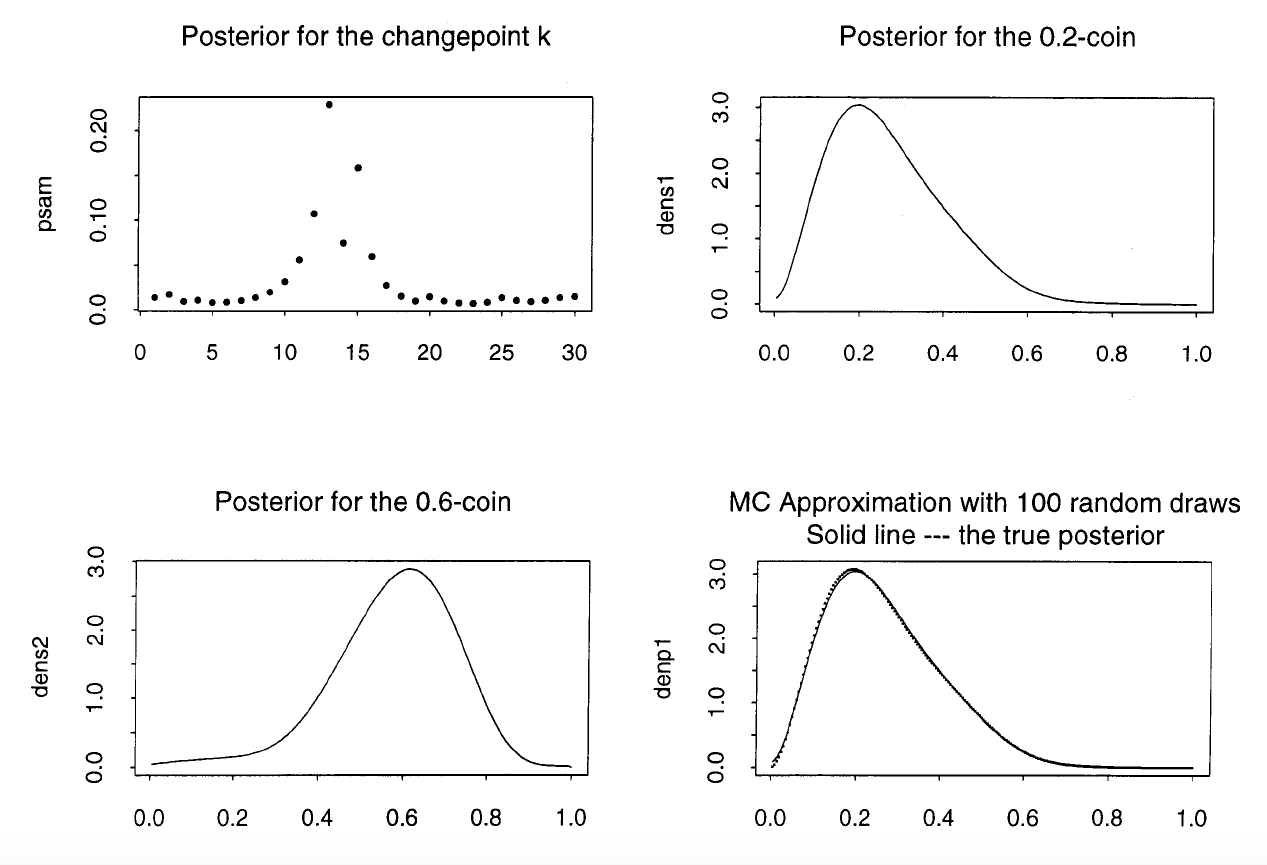
\includegraphics[scale=0.23]{LiuGraph.png}
            \caption{Liu \& Lawrence 1999}
            \label{fig:liuAndLawrence}
        \end{figure}
        % 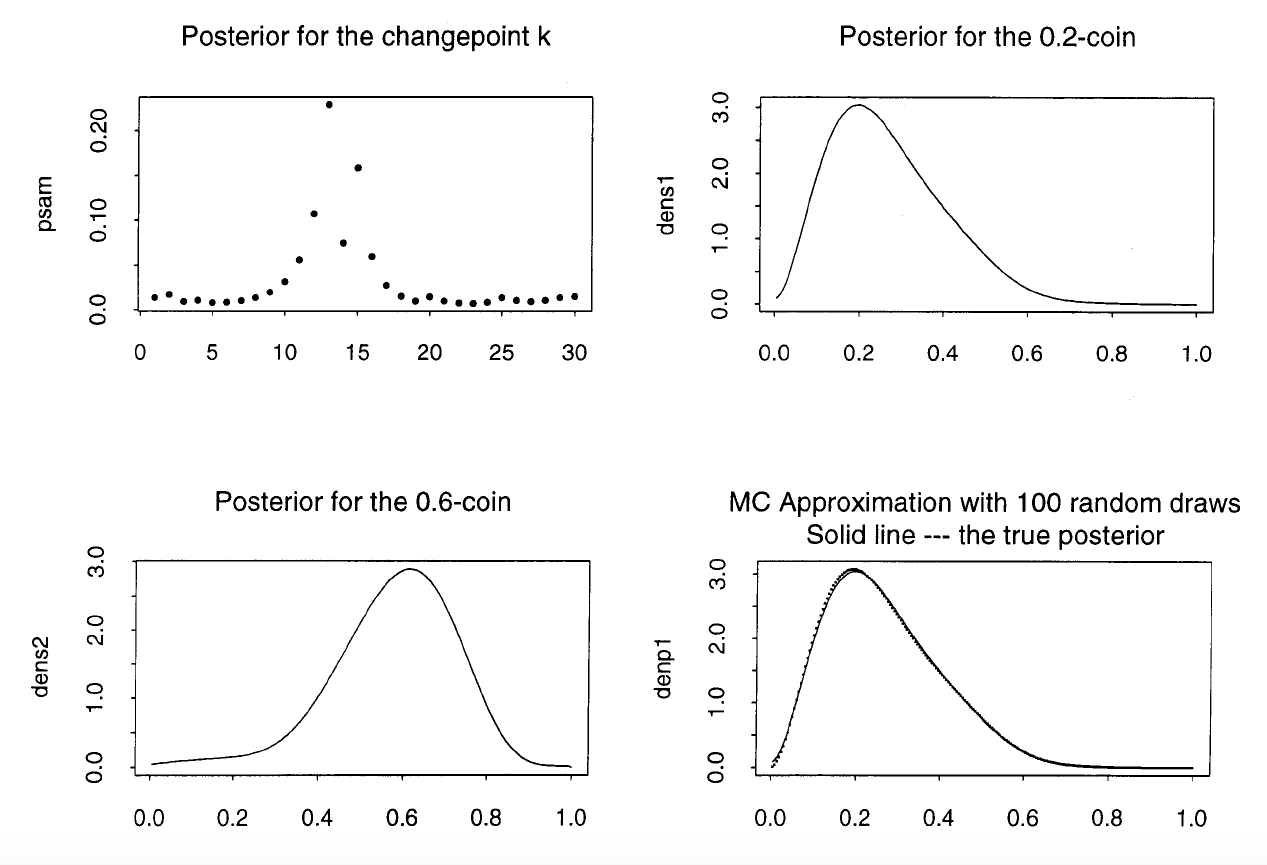
\includegraphics[scale=0.23]{LiuGraph.png}\\
        % \caption{Liu \& Lawrence 1999}
        % \end{center}
    \end{frame}
    
    \begin{frame}{Considerations for Segementation}
        In practice, sequence of interest may be something like:
            $$S = \texttt{CTCGGATTACAGTGTTTACCGCGTCTTGCG}$$
        but \textbf{much} longer. 
        
        \begin{block}{Problem}
        We can segment DNA, but how do we know what segments correspond to what we are looking for? (Enhancers)
        \end{block}
    \end{frame}
    
    \begin{frame}{Comparative Genomics}
        \begin{block}{The main idea}
            Functional regions are conserved across species
        \end{block}
    \end{frame}
    
    \begin{frame}{Unaligned Sequences}
        \begin{figure}
            \centering
            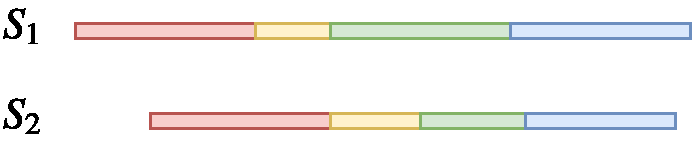
\includegraphics[width=0.9\textwidth]{UnAligned.pdf}
            \caption{Caption}
            \label{fig:unaligned}
        \end{figure}
    \end{frame}
    
    \begin{frame}{Aligned Sequences}
        \begin{figure}
            \centering
            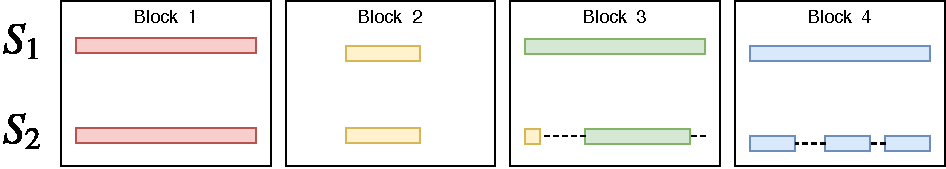
\includegraphics[width=\textwidth]{Aligned.pdf}
            \caption{Caption}
            \label{fig:aligned}
        \end{figure}
    \end{frame}
    \begin{frame}{Bayesian Segmentation and Classification}
        1s and 0s may represent matches/mismatches in an alignment
        
        \begin{align*}
            \texttt{Species 1:}&\texttt{CACATCAGCCTC}\\
            \texttt{Species 2:}&\texttt{CATACCAGTTCA}\\
            \texttt{Encoding:}&\texttt{110101110000}
        \end{align*}
        
    
    \end{frame}
    
    \begin{frame}{Encoding 2}
    Choosing to encode with a larger alphabet can include information about:
        \begin{itemize}
            \item Conservation
            \item CG content
            \item Transition/Transvertion ratio
        \end{itemize}
        \begin{align*}
            \texttt{Species 1:}&\texttt{AAAACCCCGGGGTTTTN}\\
            \texttt{Species 2:}&\texttt{ACGTACGTACGTACGT-}\\
            \texttt{Encoding:}&\texttt{abcdefghijklmnopI}
        \end{align*}
    The character \texttt{I} is ignored in change point analysis and \texttt{N} is any base.
    \end{frame}
    
    \begin{frame}{Change Point}
    The earlier model is extended by:
        \begin{itemize}
            \item Introducing segment classes. 
            \item Allocating segments to segment classes.
            \item Including the number of change points into the inference.
            \item Including hyper-parameters into the inference.
        \end{itemize}
    \end{frame}
    
    \begin{frame}{Segment classes}
        Let $S$ be a sequence, comprised of the concatenation of $s_1,s_2,\ldots,s_k$ segments. 
        
            \begin{itemize}
                \item Instead of saying $s_i$ is conserved or not.
                \item Assign $s_i$ to one of $T$ evolutionary rate classes.
            \end{itemize}
        One of the underlying assumptions is that slower evolving regions are under some pressure to stay the same, implying function.
    \end{frame}
    
    \begin{frame}{The Model}
    \begin{columns}
    \begin{column}{0.5\textwidth}
    \begin{itemize}
        \item $\pi$ - Pr. assigning segments to a class.
        \item $g$ - The class to which each segment is allocated to. 
        \item $\alpha$ - parameters for Dirichlet dist.
        \item $\theta\sim Dir(\theta;\alpha)$ for generating a character in a segment.
        \item $C$ - location of change points.
        \item $\phi$ - parameter for the distribution of change point positions.
        \item $K$ - No. change points.
        \item $S$ - Sequence.
    \end{itemize}
    \end{column}
    \begin{column}{0.5\textwidth}  %%<--- here
    \begin{center}
    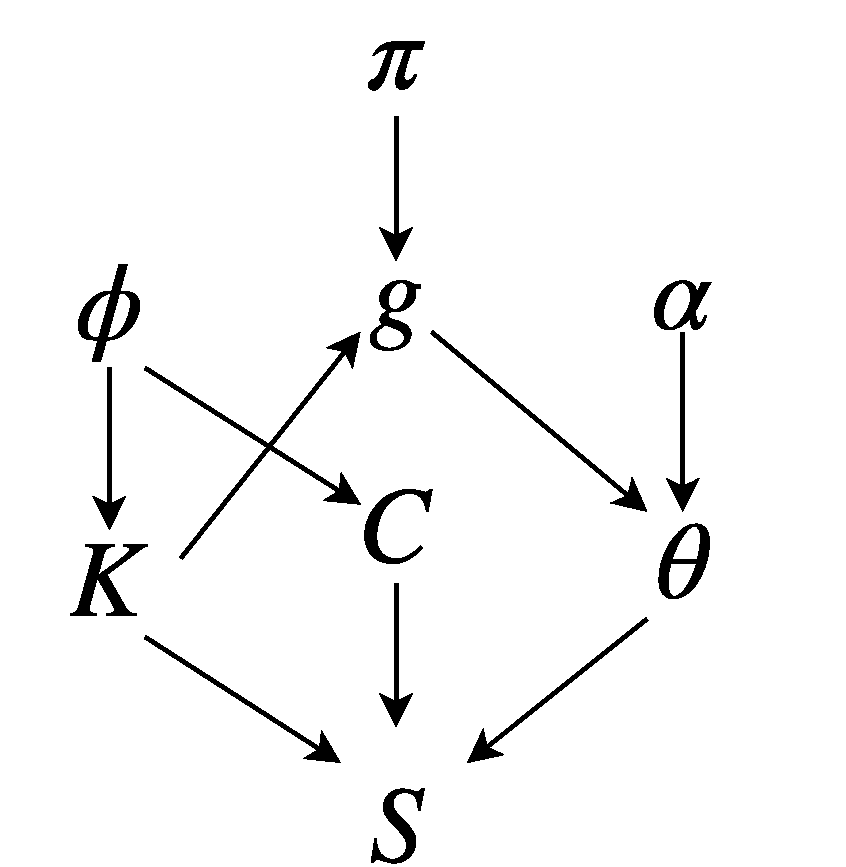
\includegraphics[width=0.9\textwidth]{condDep.pdf}\\
    \caption{Conditional dependencies of Change Point. Quantities at the head of an arrow are conditionally dependent on quantities at the tail.}
    \end{center}
\end{column}
\end{columns}
    \end{frame}
    \begin{frame}{Other Considerations}
        \begin{itemize}
            \item Conventional Gibbs sampling is not sufficient for MCMC sampling for ChangePt.
                \pause
                \begin{itemize}
                    \item Require Generalized Gibbs sampling since the dimension of the space we sample from is non-constant.
                \end{itemize}
                \pause
            \item Model selection for the number of segment classes $T$.
                \pause
                \begin{itemize}
                    \item Based on information criteria (AIC, BIC, DICV).
                \end{itemize}
        \end{itemize}
        
    
        
    \end{frame}
    
    \begin{frame}{Optimal Combination of Binary Classifiers}
        How do we know that the segments identified are \emph{interesting}? 
        
        \begin{itemize}
            \item Conservation
            \item Conservation and GC content
            \item DNase-seq footprint regions
            \item ChIP-seq regions
            \item DNase I hypersensitivity sites
        \end{itemize}
    \end{frame}
    
    \begin{frame}{Where to go from here}
        \begin{itemize}
            \item The incorporation of new data types. (eg. DNA methylation data)
            \item Incorporation of number of segment classes into inference.
            \item Perhaps alignment-free methods are the way to go.
        \end{itemize}
    \end{frame}
    
\end{document} 